%\documentclass[class=article, float=false, crop=false]{standalone}
%\usepackage{standalone}
%\usepackage{varioref}

%\documentclass[10pt,letterpaper]{article}
%
%\input{error_control_of_enhanced_sampling-header}
%\begin{document}

%\newlength{\heightMinusFoot}
%\setlength{\heightMinusFoot}{\textheight-2cm}

\section{Figures}

%\tracingmacros=1
\begin{figure}[h]
    \begin{center}
    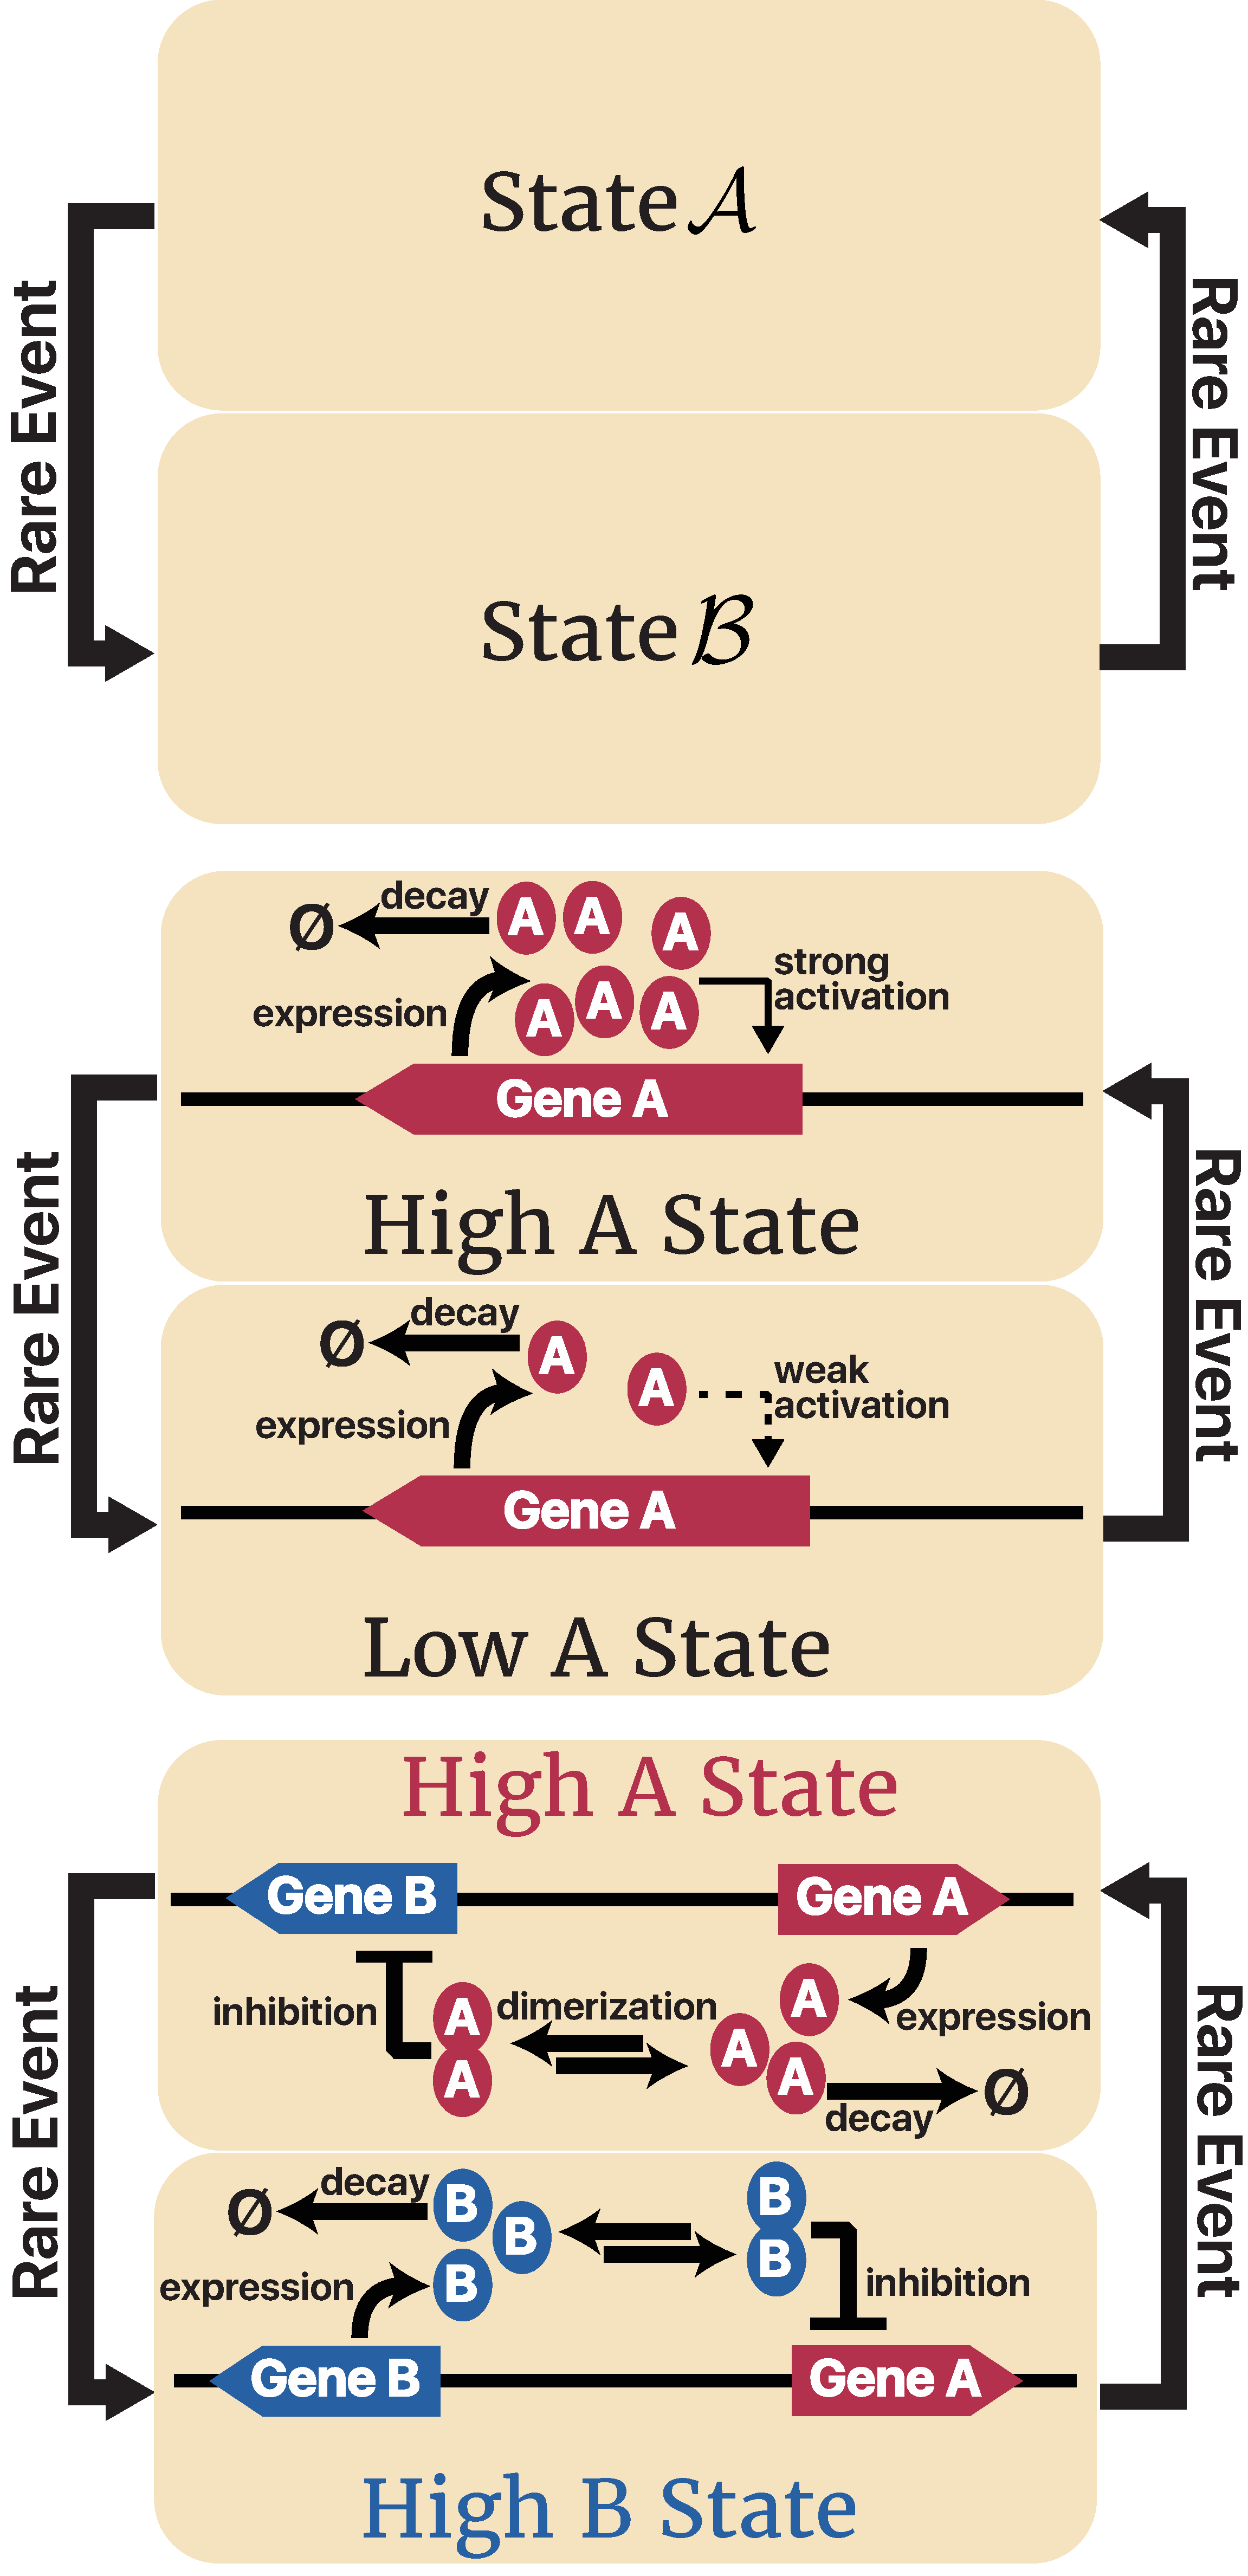
\includegraphics[width=8.45cm,height=\textheight,keepaspectratio]{{eces_chapter/model_schematics/schematic_composite_vertical}.pdf}
    \end{center}
%    \tracingmacros=1
    \caption{Schematics of the model systems investigated. \subplotcap{top} The \remname{} (\remabbrev{}, see \secref{sec:rem} and \tableref{tab:rem} for complete details). \subplotcap{middle} \srgname{} (\srgabbrev{}, see \secref{sec:srg} and \tablerefTwo{tab:srg_reactions}{tab:srg}). \subplotcap{bottom} \gtsname{} (\gtsabbrev{}, see \secref{sec:gts} and supplemental Table S1.}
%    \tracingmacros=0
    \label{fig:model_schematics}
\end{figure}
\clearpage
%\tracingmacros=0

%\begin{figure}[h]
%    \begin{center}
%        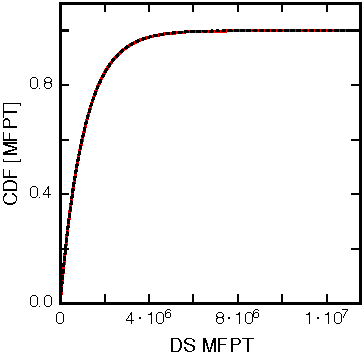
\includegraphics{{Figures/brute_force_mfpt_cdf}.pdf}
%    \end{center}
%    \caption{The empirical cumulative distribution function (shown in red) of $10^{5}$ first passage times gathered using \abr{DS}. The best fit exponential distribution, calculated using Maximum Likelihood Estimation, is shown as a black dotted line. The empirical CDF and the fitted exponential distribution appear to overlap almost exactly at the scale depicted in the above figure. All data was collected from simulations of the genetic toggle switch at $\theta=1.0$.}
%    \label{fig:brute_force_mfpt_cdf}
%\end{figure}
%\clearpage
%
%\begin{figure}[h]
%    \begin{center}
%        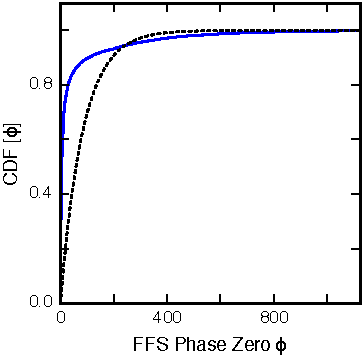
\includegraphics{{Figures/ffpilot_phase_zero_dwell_time_cdf}.pdf}
%    \end{center}
%    \caption{The empirical cumulative distribution function (shown in blue) of $10^{5}$ waiting times in between forward flux events during FFS phase 0. The best fit exponential distribution, calculated using Maximum Likelihood Estimation, is shown as a black dotted line. The moments of the empirical CDF and the best fit exponential distribution are not in good agreement. All data was collected from simulations of the genetic toggle switch at $\theta=1.0$.}
%    \label{fig:ffpilot_phase_zero_dwell_time_cdf}
%\end{figure}
%\clearpage

\begin{figure}[h]
    \begin{center}
        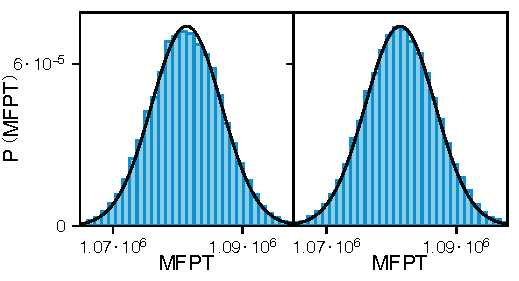
\includegraphics{{eces_chapter/Figures/toy_model_estimator_distributions_-_eg_1.0e-02_-_theta_1.0e+00_-_samples_1.6e5}.pdf}
    \end{center}
    \caption{\abr{MFPT} estimates for \abr{REM} calculated using (left) \abr{DS} and (right) \abr{FFPilot}. Shown are (blue bars) binned $\mfpttrue$ estimates from $1.6\cdot 10^5$ simulations with a 1\% error goal and (black lines) $\mfpttrue$ estimate distributions from \eqref{eq:fpt_clt_distribution} and \eqref{eq:PWest_asymptotic_dist}, respectively.}
    \label{fig:toy_model_estimator_distributions}
\end{figure}
\clearpage

\begin{figure}[h]
    \begin{center}
        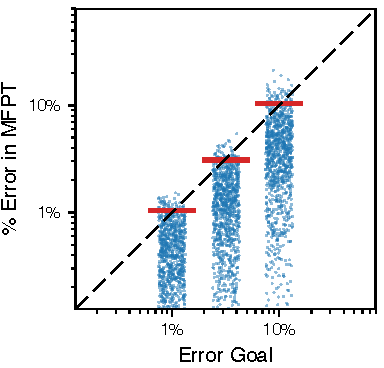
\includegraphics{{eces_chapter/Figures/toy_model_acutal_error_vs_predicted_error_-_cropped}.pdf}
    \end{center}
    \caption{Actual error vs error goal of \abr{FFPilot} simulations of the \abr{REM}. Each strip shows the \abr{MFPT} estimation error from (blue dots) 1000 independent \abr{FFPilot} simulations and (red lines) the 95th percentiles of the errors. Jitter was added to the x-position of the dots for visualization.}
    \label{fig:toy_model_actual_error_vs_predicted_error}
\end{figure}
\clearpage

%\begin{figure}[h]
%    \begin{center}
%        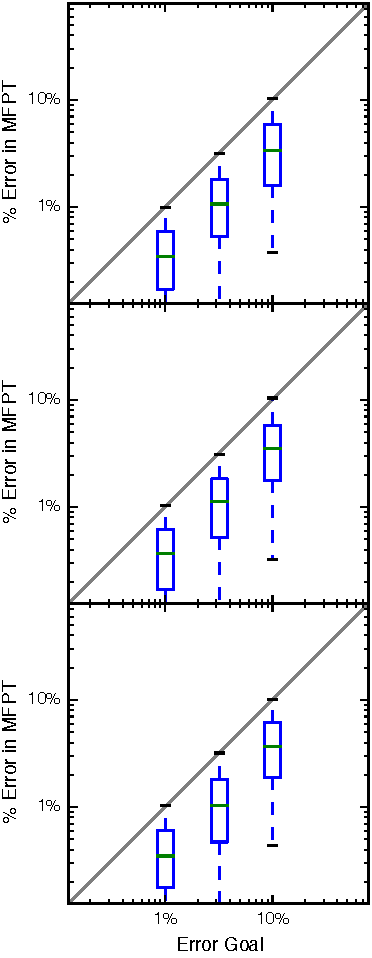
\includegraphics{{eces_chapter/Figures/toy_model_acutal_error_vs_predicted_error_-_boxplot}.pdf}
%    \end{center}
%    \caption{Box plots of actual error vs error goal for 9000 simulations of the simplified genetic toggle switch model. Each box is based on 1000 simulations run at the particular error goal corresponding to the position on the x axis. Each separate subplot is from a model with a different value of $\theta$ (from top to bottom, $\theta = 0.1, 1, 10$). All subplots are in log scale.}
%    \label{fig:toy_model_actual_error_vs_predicted_error_-_boxplot}
%\end{figure}
%\clearpage
%
%
%\begin{figure}[h]
%    \begin{center}
%        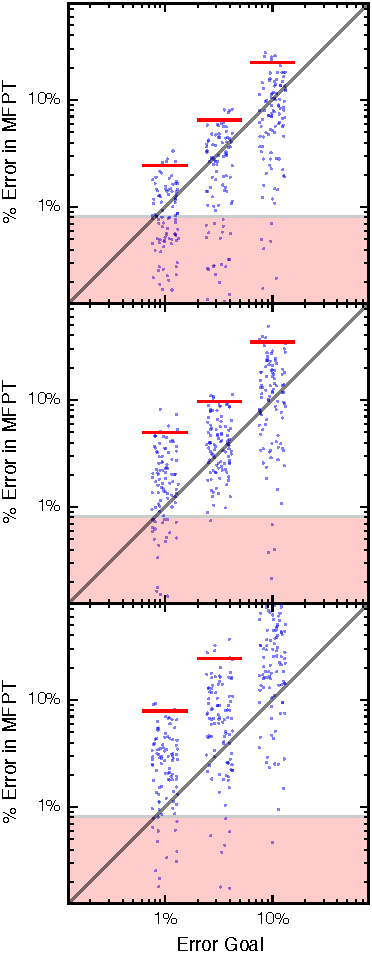
\includegraphics{{eces_chapter/Figures/cme_model_percent_error_vs_error_goal_-_reps_100}.pdf}
%    \end{center}
%    \caption{Results from 900 \abr{FFPilot} simulations. Specifically, strip plots showing a comparison of percent error vs error goal in estimated MFPT values from full CME simulations of different variants of the genetic toggle switch (from top to bottom, $\theta=0.1, 1, 10$). The 95th percentile of the error in the \abr{FFPilot} results at each of the different error goals is marked with a red line. Percent error was determined via a comparison of \abr{FFPilot} results with a highly accurate set of equivalent results produced using \abr{DS} ($10^5$ replicates). The 99\% confidence interval of the \abr{DS} comparison data set is marked as a red interval.}
%    \label{cme_model_percent_error_vs_error_goal}
%\end{figure}
%\clearpage
%
%
%\begin{figure}[h]
%    \begin{center}
%        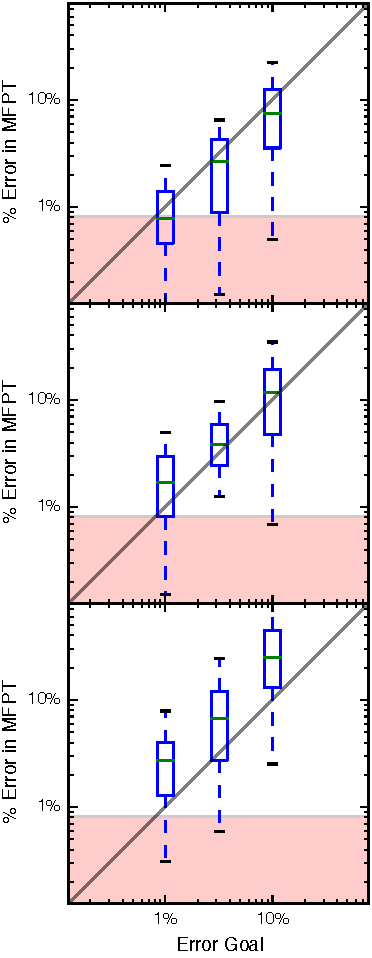
\includegraphics{{eces_chapter/Figures/cme_model_percent_error_vs_error_goal_-_reps_100_-_boxplot}.pdf}
%    \end{center}
%    \caption{Results from 900 \abr{FFPilot} simulations. Specifically, box and whisker plots showing a comparison of percent error vs error goal in estimated MFPT values from full CME simulations of different variants of the genetic toggle switch (from top to bottom, $\theta=0.1, 1, 10$). The green line marks the median of the distribution of errors at each different error goal, and the whiskers mark the 5th and 95th percentiles. Percent error was determined via a comparison of \abr{FFPilot} results with a highly accurate set of equivalent results produced using \abr{DS} ($10^5$ replicates). The 99\% confidence interval of the \abr{DS} comparison data set is marked as a red interval.}
%    \label{cme_model_percent_error_vs_error_goal_boxplot}
%\end{figure}
%\clearpage

\begin{figure}[h]
    \begin{center}
        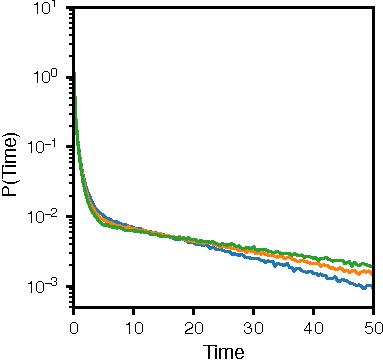
\includegraphics{{eces_chapter/Figures/name_srg_-_ffpilot_phase_zero_dwell_time_dist}.pdf}
    \end{center}
    \caption{Waiting times between forward crossing events during phase 0 of forward flux simulations of the \abr{SRG} models. Each line shows a distribution calculated from $10^6$ samples from a single phase 0 trajectory of (blue) $\SRGSLOWEST$, (orange) $\SRGSLOWER$ , and (green) $\SRGSLOW$.}
    \label{fig:name_srg_-_ffpilot_phase_zero_dwell_time_dist}
\end{figure}
\clearpage

\begin{figure}[h]
    \begin{center}
        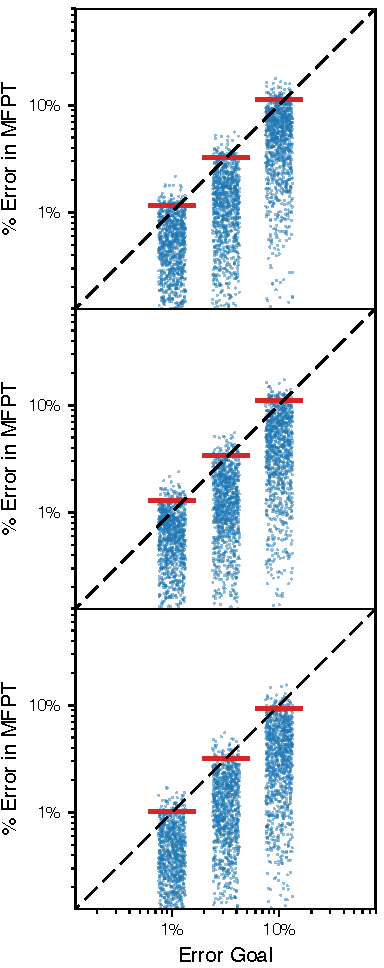
\includegraphics{{eces_chapter/Figures/name_h_-_stage_percent_error_-_error_goal_all_-_h_all}.pdf}
    \end{center}
    \caption{Actual error vs error goal of \abr{FFPilot} simulations for (top) $\SRGSLOWEST$, (middle) $\SRGSLOWER$, and (bottom) $\SRGSLOW$. Each strip shows (blue dots) 1000 independent \abr{FFPilot} simulations and (red lines) the 95th percentiles of the errors.}
    \label{fig:name_srg_-_error_goal_test_complete_-_h_all}
\end{figure}
\clearpage

\begin{figure}[h]
    \begin{center}
        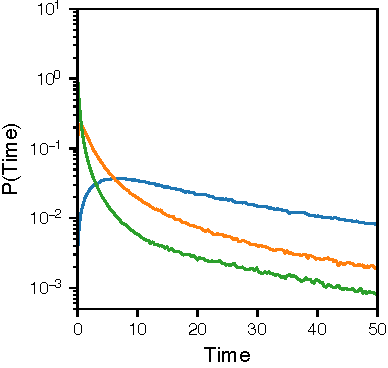
\includegraphics{{eces_chapter/Figures/name_gts_-_ffpilot_phase_zero_dwell_time_dist}.pdf}
    \end{center}
    \caption{Waiting times between forward crossing events during phase 0 of \abr{FFS} simulations of the \abr{GTS} models. Each line shows a distribution calculated from $10^6$ samples from a single phase 0 trajectory of (blue) $\GTSSLOWEST$, (orange) $\GTSSLOWER$, and (green) $\GTSSLOW$.}
    \label{fig:name_gts_-_ffpilot_phase_zero_dwell_time_dist}
\end{figure}
\clearpage

\begin{figure}[h]
    \begin{center}
        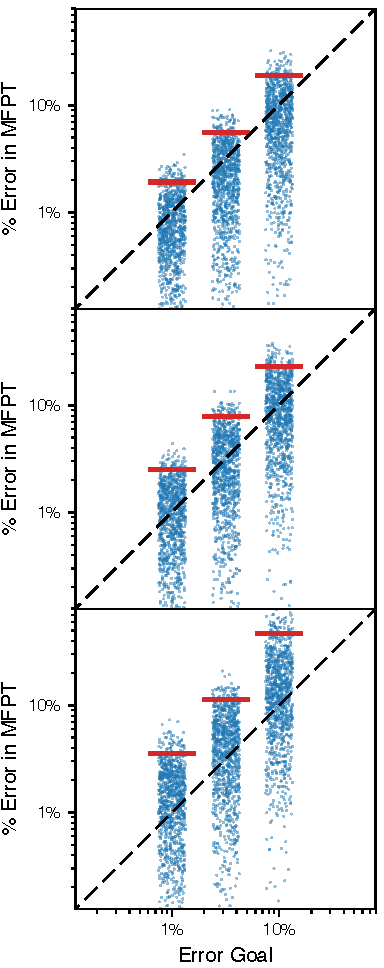
\includegraphics{{eces_chapter/Figures/name_theta_-_stage_percent_error_-_error_goal_all_-_theta_all}.pdf}
    \end{center}
    \caption{Actual error vs error goal of \abr{FFPilot} simulations for (top) $\GTSSLOWEST$, (middle) $\GTSSLOWER$, and (bottom) $\GTSSLOW$. Each strip shows (blue dots) 1000 independent \abr{FFPilot} simulations and (red lines) the 95th percentiles of the errors.}
    \label{fig:name_gts_-_error_goal_test_complete_-_theta_all}
\end{figure}
\clearpage

\begin{figure}[h]
    \begin{center}
        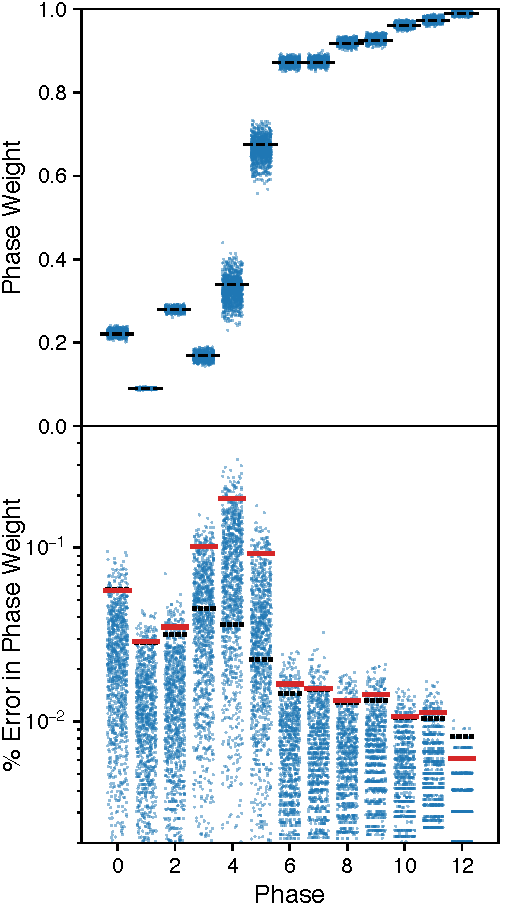
\includegraphics{{eces_chapter/Figures/name_theta_-_phase_weight_percent_error_-_error_goal_1.0e-01_-_theta_1.0e+01_enlarged}.pdf}
    \end{center}
    \caption{$\GTSSLOW$ phase weight estimates and errors. \subplotcap{top} The phase weights as estimated by (blue dots) 1000 independent \abr{FFPilot} simulations run to a 10\% error goal. The dashed black lines show the phase weights from an FFPilot simulation with a 0.1\% error goal. \subplotcap{bottom} The blue dots show the percent error of each phase weight estimate given in the top subplot, relative to the 0.1\% error goal simulation. Also shown are (red lines) the observed 95th error percentiles, and (dashed black lines) the expected 95th error percentiles.}
    \label{fig:name_gts_-_phase_weight_percent_error_-_error_goal_1.0e-01_-_theta_1.0e+01}
\end{figure}
\clearpage

\begin{figure}[h]
    \begin{center}
        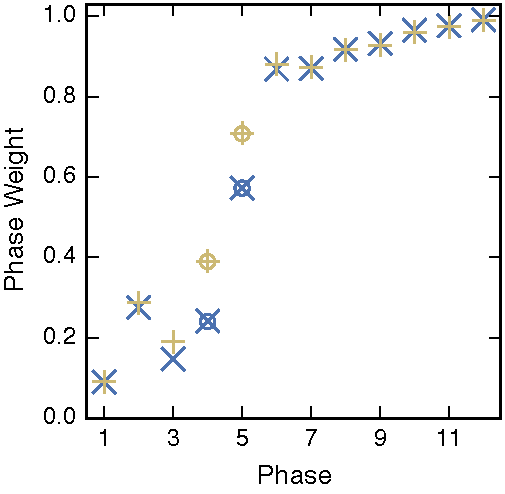
\includegraphics{{eces_chapter/Figures/name_gts_-_phase_weights_-_rep_6_8_-_theta_1.0e+01_-_enlarged}.pdf}
    \end{center}
    \caption{The phase weights of two replicates: (blue x) Replicate 6 and (gold +) Replicate 8, from a $\GTSSLOW$ \abr{FFPilot} simulation run to an error goal of 10\%. Circles show weights for phases 4 and 5 calculated via an alternative method using \eqref{eq:reconstituted_phase_weights}.}
    
    %The phase weights of phases 4 and 5 were recalculated using an alternative method that only used the landscapes assembled by the replicates, rather than the outcomes of the simulations in the given phase. These recalculated phase weights are shown as hollow circles (Replicate 6 in blue, Replicate 8 in gold).}
%    \caption{The phase weights of two replicates, Replicate 6 \inlinelegend{{eces_chapter/Figures/name_gts_-_phase_weights_-_rep_6_8_-_theta_1.0e+01_marker_0}.pdf} and Replicate 8 \inlinelegend{{eces_chapter/Figures/name_gts_-_phase_weights_-_rep_6_8_-_theta_1.0e+01_marker_1}.pdf}, of an \abr{FFPilot} simulation of the genetic toggle switch (with $\theta=10$) run to an error goal of 10\%. In phases 4 and 5, which are the two phases leading up to the midpoint of the transition path, the phase weights of these two replicates diverge greatly. The phase weights of phases 4 and 5 were recalculated using an alternative method that only used the landscapes assembled by the replicates, rather than the outcomes of the simulations in the given phase. These recalculated phase weights are shown as hollow circles (Replicate 6 \inlinelegend{{eces_chapter/Figures/name_gts_-_phase_weights_-_rep_6_8_-_theta_1.0e+01_marker_2}.pdf}, Replicate 8 \inlinelegend{{eces_chapter/Figures/name_gts_-_phase_weights_-_rep_6_8_-_theta_1.0e+01_marker_3}.pdf}}).
    \label{fig:name_gts_-_phase_weights_-_rep_6_8_-_theta_1.0e+01}
\end{figure}
\clearpage

\begin{figure}[h]
    \begin{center}
        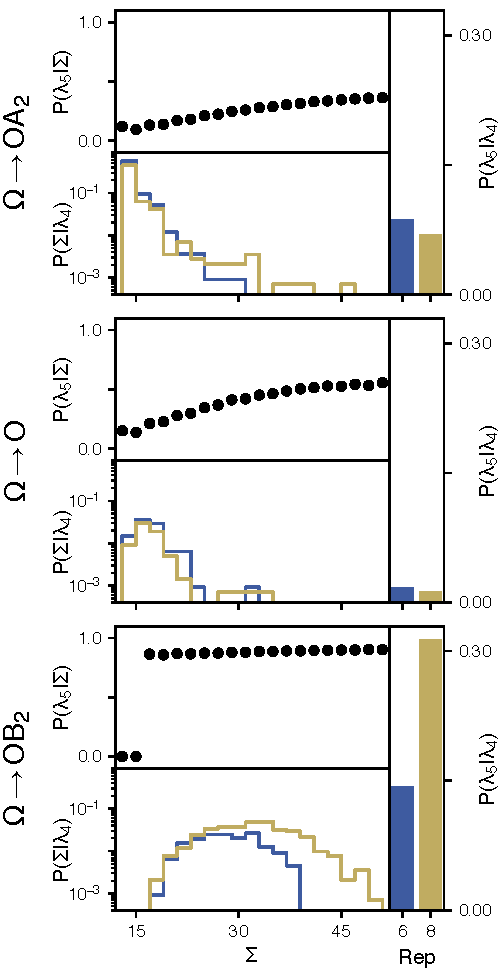
\includegraphics{{eces_chapter/Figures/name_gts_-_phase_weight_4_split_by_operator_-_rep_6_8_-_theta_1.0e+01_-_dists_-_one-col}.pdf}
%        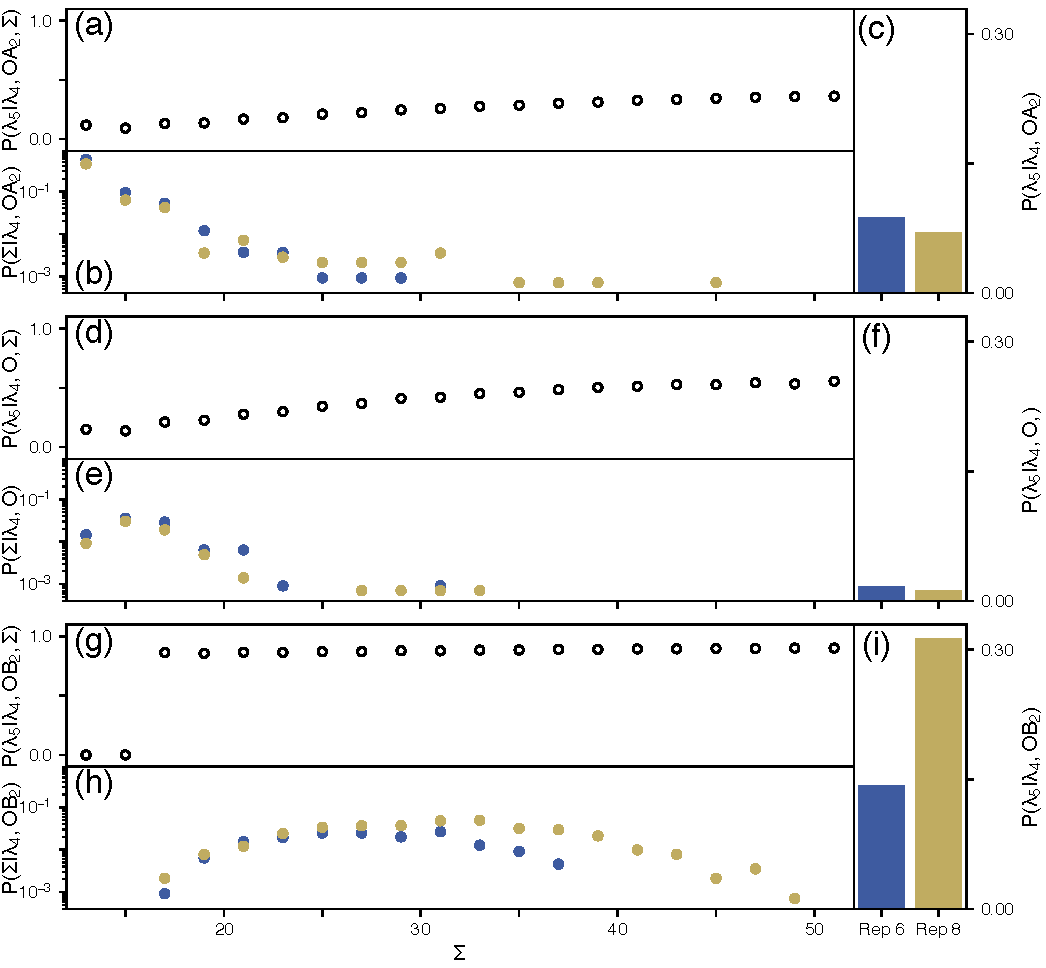
\includegraphics{{eces_chapter/Figures/name_gts_-_phase_weight_4_split_by_operator_-_rep_6_8_-_theta_1.0e+01_-_dots}.pdf}
%        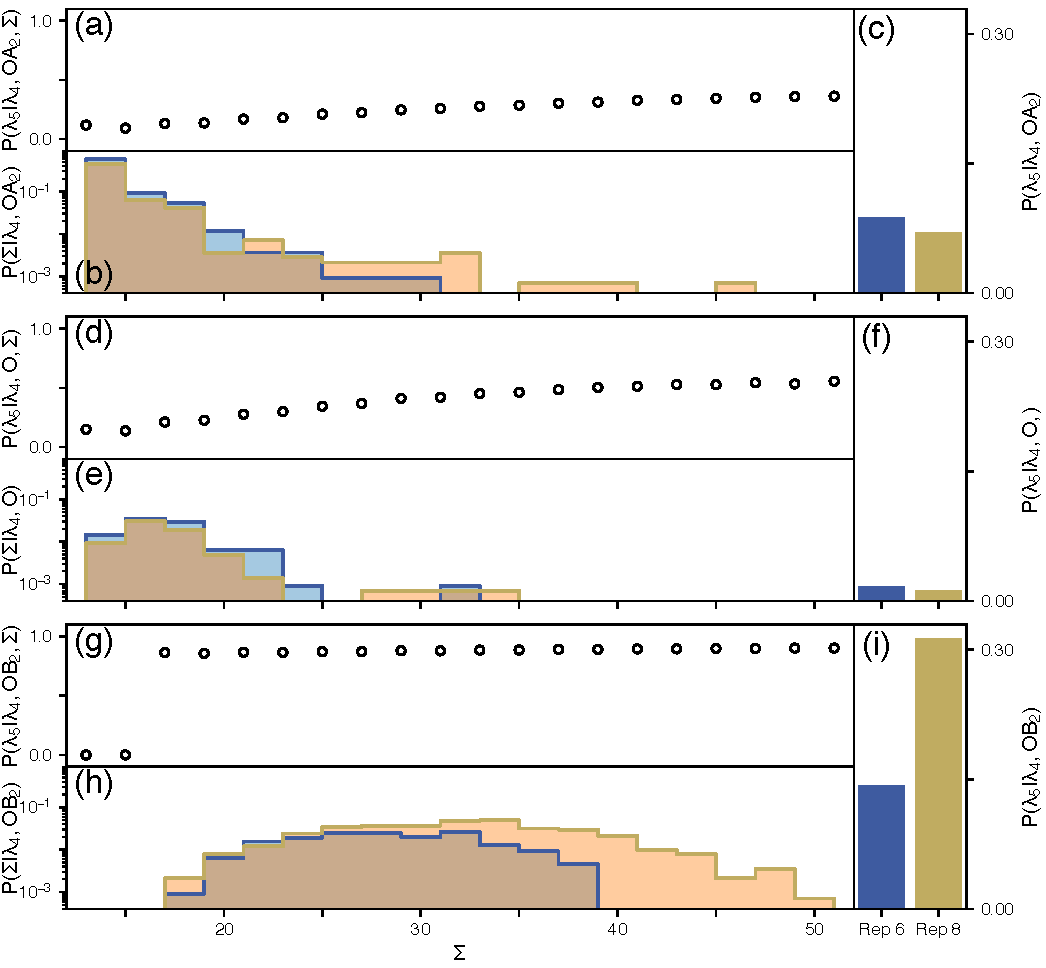
\includegraphics{{eces_chapter/Figures/name_gts_-_phase_weight_4_split_by_operator_-_rep_6_8_-_theta_1.0e+01_-_dists_filled}.pdf}
    \end{center}
    \caption{Breakout of the calculation of phase weight 5 for replicates 6 and 8. Each group of three plots show data from a slice of \abr{GTS} state space with a different $\gtsostate$, the state of the operator DNA. Each subplot within a group shows different probability data. (dots) The probability of a trajectory launched from a point on $\ifacex{4}$ fluxing forward to $\ifacex{5}$ vs the orthogonal order parameter $\gtsbpa$. (lines) The occupancy along $\gtsbpa$ at interface $\ifacex{4}$ for (blue) replicate 6 and (gold) replicate 8. (bars) The cumulative probability of fluxing forward across $\ifacex{5}$ when starting at the specified $\gtsostate$ for (blue) replicate 6 and (gold) replicate 8.}
    \label{fig:name_gts_-_phase_weight_4_split_by_operator_-_rep_6_8_-_theta_1.0e+01}
\end{figure}
\clearpage

%\begin{figure}[h]
%    \begin{center}
%        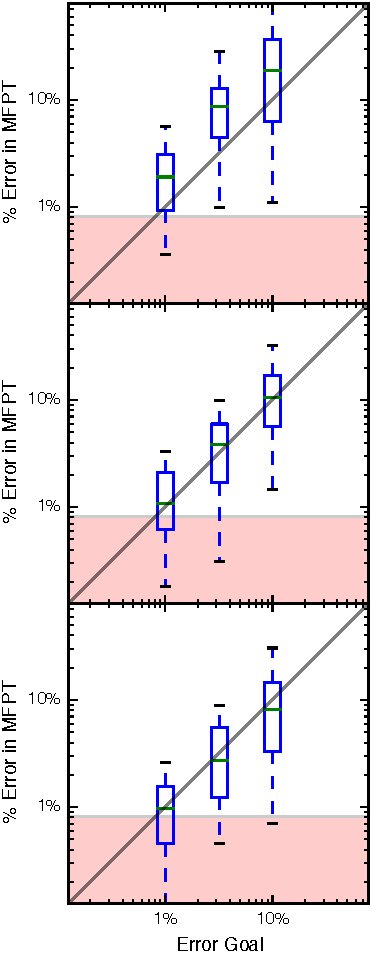
\includegraphics{{eces_chapter/Figures/cme_model_percent_error_vs_error_goal_at_different_phase_zero_mults-_reps_100_-_theta_1.0e+01_-_boxplot}.pdf}
%    \end{center}
%    \caption{Box and whisker plots showing the effect of oversampling during \abr{FFPilot} phase 0 on overall simulation accuracy. From top to bottom, the subplots show the results from 300 \abr{FFPilot} simulations (100 per error goal) of the genetic toggle switch at $\theta=10$ carried out with 1X, 10X, and 100X sampling during \abr{FFPilot} phase 0. The calculation of the percent error in the estimated MFPT was carried out with the same protocol as described in the caption of fig \ref{cme_model_percent_error_vs_error_goal_boxplot}. }
%    \label{fig:cme_model_percent_error_vs_error_goal_at_different_phase_zero_mults}
%\end{figure}
%\clearpage
%
%\begin{figure}[h]
%    \begin{center}
%        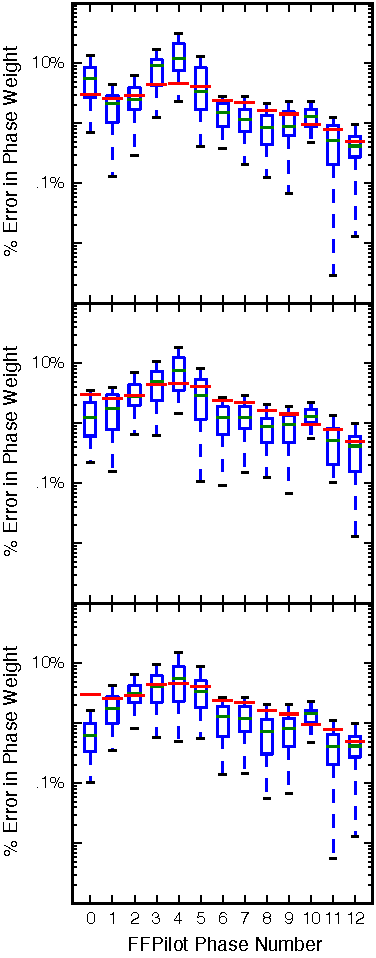
\includegraphics{{eces_chapter/Figures/ffpilot_phase_weight_percent_errors_vs_predicted_errors_-_theta_1.0e+01}.pdf}
%    \end{center}
%    \caption{Box and whisker plots showing an in-depth examination of how the errors in each of the phase weights change as more samples are taken during \abr{FFPilot} phase 0. From top to bottom, 1X, 10X, and 100X sampling during \abr{FFPilot} phase 0 was performed.   Each subplot contains data from 100 \abr{FFPilot} simulation of the genetic toggle switch at $\theta=10$ carried out with an error goal of $10\%$. \newline
%    The red lines show the predicted value for the 95th percentile of each of the phase weight error distributions. In other words, the optimizing equation predicts that the top whisker of each box will be bellow the red line, and further that if this condition is met it is likely that the error in the MFPT will also be in the desired range. However, the optimizing equation does not take the effects of landscape error directly into account.}
%    \label{fig:ffpilot_phase_weight_percent_errors_vs_predicted_errors}
%\end{figure}
%\clearpage

\begin{figure}[h]
    \begin{center}
        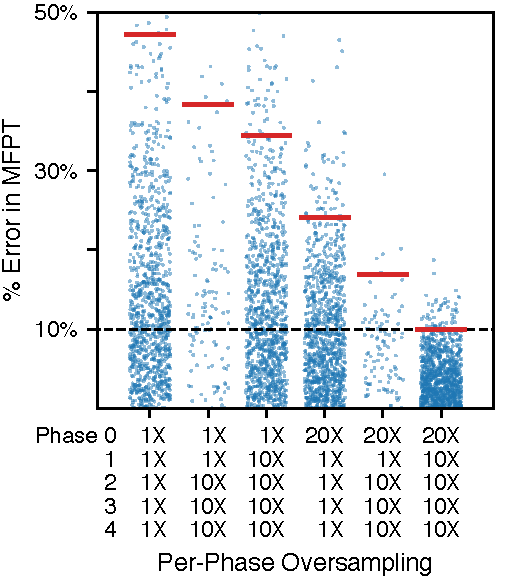
\includegraphics{{eces_chapter/Figures/name_gts_-_stage_fpt_percent_error_-_landscape_fudge_several_-_error_goal_1.0e-01_-_theta_1.0e+01_-_enlarged}.pdf}
    \end{center}
    \caption{Errors from simulations executed with various oversampling schemes. The extent of oversampling in each phase for the separate schemes is indicated beneath each column of results. All simulations were of $\GTSSLOW$ run to an error goal of 10\%. Red lines show the 95th error percentiles.}
    \label{fig:name_gts_-_stage_fpt_percent_error_-_landscape_fudge_several_-_error_goal_1.0e-01_-_theta_1.0e+01}
\end{figure}
\clearpage

\begin{figure}[h]
    \begin{center}
        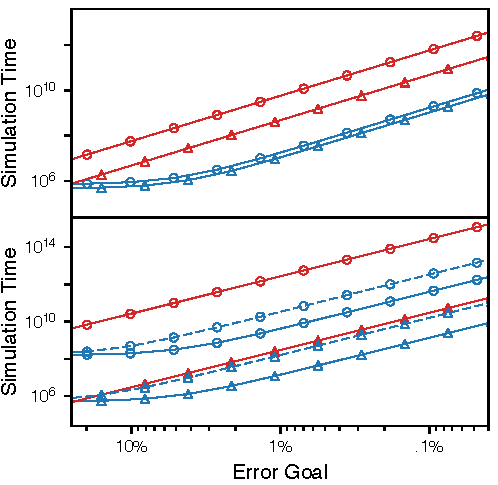
\includegraphics{{eces_chapter/Figures/name_theta_-_name_h_-_speedup_plot_-_simtime_vs_error_goal}.pdf}
    \end{center}
    \caption{Simulation time vs error goal for several \abr{SRG} and \abr{GTS} models. Simulation time was calculated using \eqref{eq:ds_cost} for (red lines) \abr{DS}, and \eqref{eq:ffpilot_cost} for (blue lines) \abr{FFPilot} and (dashed line) \abr{FFPilot} with oversampling to correct the landscape error. Parameters were taken from \tablerefTwo{tab:srg}{tab:gts}. (top) Data from (circles) $\SRGSLOWEST$ and (triangles) $\SRGSLOW$. (bottom) Data from (circles) $\GTSSLOWEST$ and (triangles) $\GTSSLOW$.}
    \label{fig:name_srg_-_speedup_plot_-_simtime_vs_moe}
\end{figure}
\clearpage

\begin{figure}[h]
    \begin{center}
        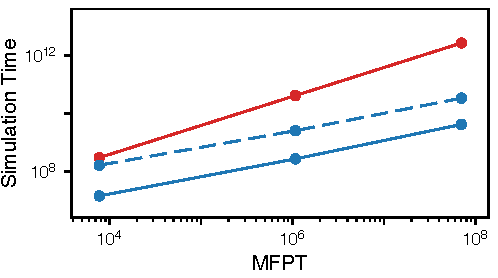
\includegraphics{{eces_chapter/Figures/name_theta_-_speedup_plot_-_simtime_vs_mfpt_-_error_goal_1.0e-02}.pdf}
    \end{center}
    \caption{Simulation time vs \abr{MFPT} for several \abr{GTS} models. Simulation times are shown for (red dots) \abr{DS}, (blue dots) \abr{FFPilot}, and (blue dots with dashed line) \abr{FFPilot} with oversampling to correct for landscape error. The simulation times shown are averaged across 1000 simulations. Connecting lines added for illustration.}
    \label{fig:name_theta_-_speedup_plot_-_simtime_vs_mfpt_-_error_goal_1.0e-02}
\end{figure}
\clearpage

%\begin{figure}[h]
%    \begin{center}
%        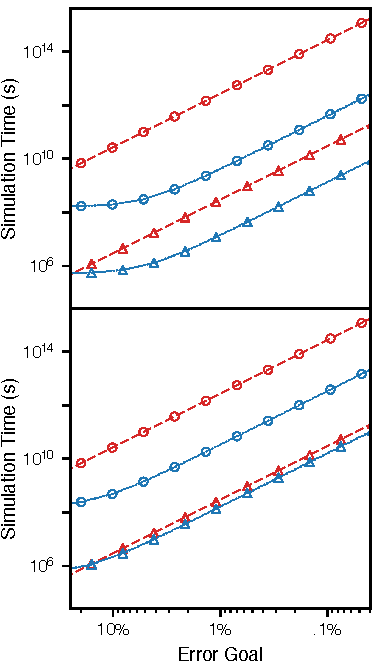
\includegraphics{{eces_chapter/Figures/name_theta_-_speedup_plot_-_simtime_vs_error_goal}.pdf}
%    \end{center}
%    \caption{A comparison of how the simulation time scales with respect to error goal for the genetic toggle switch models $\GTSSLOW$ (triangles) and $\GTSSLOWEST$ (circles). The simulation time for both \abr{DS} (red lines) and \abr{FFPilot} Sampling (blue lines) are shown. The results were derived from \eqrefTwo{eq:ds_sim_time}{eq:ffpilot_cost}. The equation was parameterized from the mean results of 1000 simulations of each model run at a 1\% error goal. The results without any correction for landscape error are shown in the top subplot, and the results with the landscape corrections determined in \secref{sec:oversampling} are shown in the bottom subplot.}
%    \label{fig:name_theta_-_speedup_plot_-_simtime_vs_error_goal}
%\end{figure}
%\clearpage
%
%\begin{figure}[h]
%    \begin{center}
%        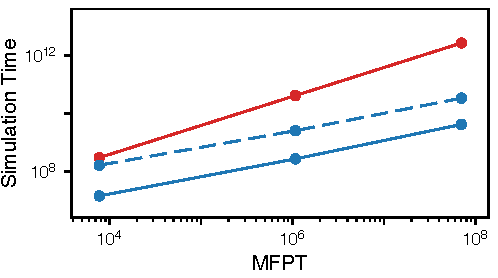
\includegraphics{{eces_chapter/Figures/name_theta_-_speedup_plot_-_simtime_vs_mfpt_-_error_goal_1.0e-02}.pdf}
%    \end{center}
%    \caption{A comparison of how the simulation time required for \abr{DS} (red circles) and \abr{FFPilot} Sampling (blue circles) scale with respect to the \abr{MFPT} of the various versions of the \gtsname{}. The rate at which a given version of the \gtsname{} transitions from state to state can be tuned using the relative protein churn rate parameter $\theta$. The results were derived from \eqref{eq:optimizing_equation_general_form}. The equation was parameterized from empirical results drawn from 1000 \abr{FFPilot} simulations of the \gtsname{} models run at a $\%1$ error goal.}
%    \label{fig:name_theta_-_speedup_plot_-_simtime_vs_mfpt_-_error_goal_1.0e-02}
%\end{figure}
%\clearpage
%
%
%\begin{figure}[h]
%    \begin{center}
%        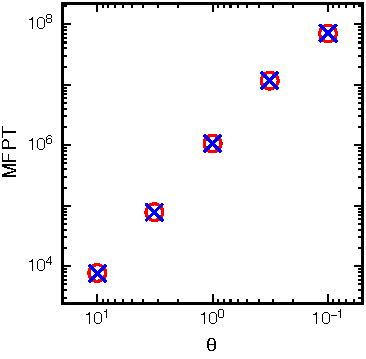
\includegraphics{{eces_chapter/Figures/ffpilot_bf_mfpt_vs_theta_scatter_-_eg_1.0e-02}.pdf}
%    \end{center}
%    \caption{Comparison of \abr{MFPT} values calculated with \abr{DS} and with \abr{FFPilot}. Both methods were run with a $1\%$ error goal, and the \abr{FFPilot} simulations were run with 10X phase 0 sampling. Each data point is the average of 5 simulations, and error bars are not shown because they are too small to see.}
%    \label{fig:mfpt_vs_theta}
%\end{figure}
%\clearpage
%
%\begin{figure}[h]
%    \begin{center}
%        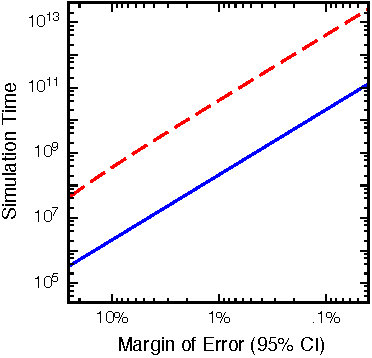
\includegraphics{{eces_chapter/Figures/toy_model_simulation_time_scaling_with_percent_error}.pdf}
%    \end{center}
%    \caption{A comparison of how the simulation time required for \abr{DS} (red dashed line) and \abr{FFPilot} Sampling (blue line) scale with respect to error goal. The results were derived from \eqref{eq:optimizing_equation_general_form}. The equation was parameterized from empirical results drawn from simulations of the full CME model of the genetic toggle switch. The parameters for each individual data point were generated from the average fit of the results of 5 simulations run at a $\%1$ error goal.}
%    \label{fig:toy_model_simulation_time_scaling_with_percent_error}
%\end{figure}
%\clearpage
%
%\begin{figure}[h]
%    \begin{center}
%        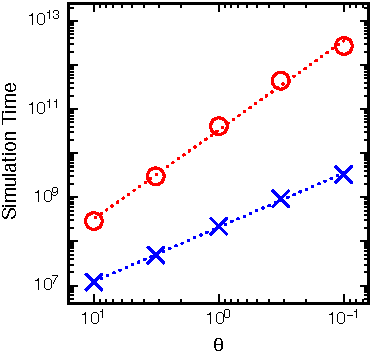
\includegraphics{{eces_chapter/Figures/ffpilot_bf_simulation_time_vs_theta_scatter}.pdf}
%    \end{center}
%    \caption{A comparison of how the simulation time required for \abr{DS} (red circles) and \abr{FFPilot} Sampling (blue Xs) scale with respect to the relative protein churn rate parameter $\theta$. Power law fits to the data are shown as dotted lines. Smaller values of $\theta$ result in a version of the genetic toggle switch that transitions more slowly from state to state, whereas larger values of $\theta$ cause it transition more frequently. The results were derived from \eqref{eq:optimizing_equation_general_form}. The equation was parameterized from empirical results drawn from simulations of the full CME model of the genetic toggle switch. The parameters for each individual data point were generated from the average fit of the results of 5 simulations run at a $\%1$ error goal.}
%    \label{fig:simulation_time_vs_theta}
%\end{figure}
%\clearpage
%
%\begin{figure}[h]
%    \begin{center}
%        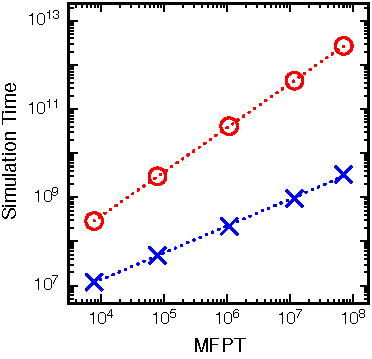
\includegraphics{{eces_chapter/Figures/ffpilot_bf_simulation_time_vs_mfpt_scatter}.pdf}
%    \end{center}
%    \caption{A comparison of how the simulation time required for \abr{DS} (red circles) and \abr{FFPilot} Sampling (blue Xs) scale with respect to the \abr{MFPT} of the various versions of the genetic toggle switch. Power law fits to the data are shown as dotted lines. The rate at which a given version of the genetic toggle switch transitions from state to state can be tuned using the relative protein churn rate parameter $\theta$. The results were derived from \eqref{eq:optimizing_equation_general_form}. The equation was parameterized from empirical results drawn from simulations of the full CME model of the genetic toggle switch. The parameters for each individual data point were generated from the average fit of the results of 5 simulations run at a $\%1$ error goal.}
%    \label{fig:simulation_time_vs_mfpt}
%\end{figure}
%\clearpage


%\input{error_control_of_enhanced_sampling-figures_roundfile}

%\end{document}